\begin{frame}
\begin{block}{topological sheaf on a two-point space}
\centering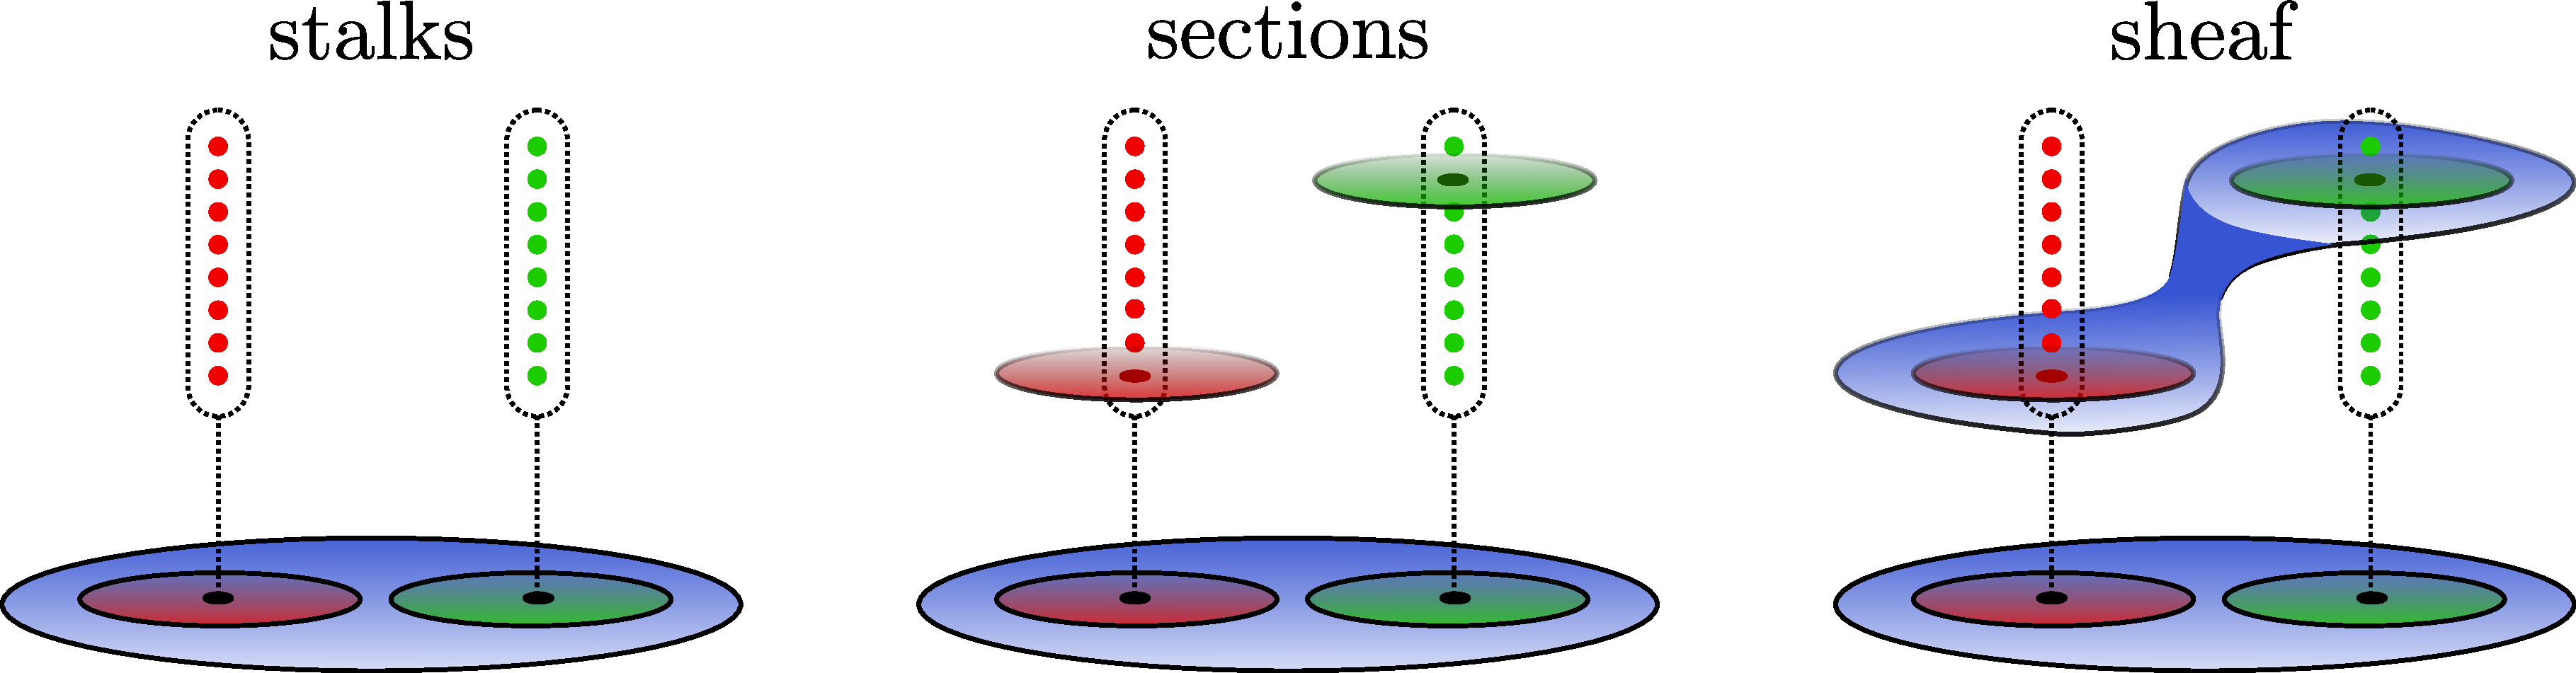
\includegraphics[width=1.0\textwidth]{fig/sheafex.pdf}
\end{block}
\begin{block}{}
An \href{http://en.wikipedia.org/wiki/Talk:Sheaf\_(mathematics)\#Some\_visualization}{analogous situation} holds for (directed) (hyper-)graphs but it is currently difficult to visualize. Future work on {\it graph transformations} may incorporate a method of directly visualizing sheaves of graphs.
\end{block}
%\begin{block}{sheaf}
%All
%\end{block}
\end{frame}

% 1. Visualising a sheaf in terms of stalks over each point of the space
% 2. Particular sections (associated to a germ of the stalk) corresponding to each of the red and green open sets of the space.
% 3. Gluing together two sections to create a section of the larger open set that they provide a cover of.